\documentclass[]{article}
\usepackage{graphicx}

%opening
\title{Parallellisme - Project report}
\author{Hans Van der Ougstraete}

\begin{document}

\maketitle
\clearpage
\tableofcontents
\clearpage

\section{Implementatie}

\subsection{Fase 1}
Fase 1 is opgedeeld in twee delen, het eerste deel maakt een lijst met relevante businesses door in de base case de evaluaterevalence methode uit SequentialSearch aan te roepen. De Yelpdata wordt dus in stukken opgedeeld tot het kleinste deel een business is. Deze lijst wordt in het tweede deel aan de hand van een parallele mergesort gesorteerd. Deze code is terug te vinden in de ParallelSearch klasse.
\subsection{Fase 2}
In progress
\section{Evaluatie}
De benchmarks op eigen computer (quad core i5-2300 @2.80GHz) zijn 3 maal uitgevoerd. Voor SequentialSearch, ParallelSearch met 2 workers en ParallelSearch met 4 workers. Dit telkens 1500 keer. Het weergeven van de resultaten is per preset zo kan men vergelijken tussen de drie verschillende benchmarks voor 1 bepaalde preset.
Hier bespreek ik de resultaten en manier van werken in het algemeen. Ik denk dat ik ga kiezen voor een boxplot per preset voor seq, 2p en 4p. 
\subsection{Fase 1}

\begin{figure}[h]
	\centering
	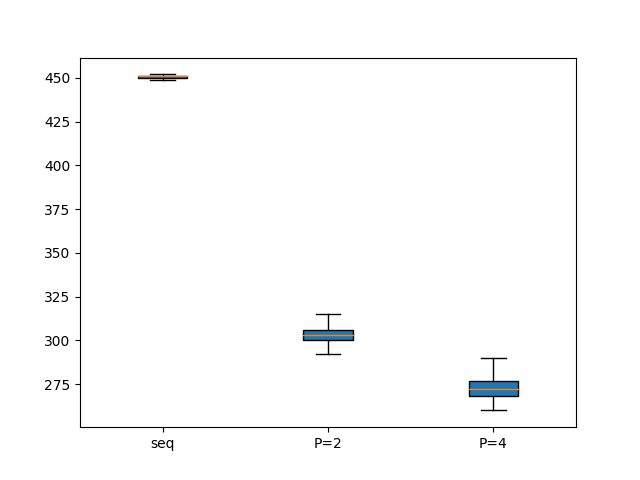
\includegraphics[width=0.7\linewidth]{Preset_1}
	\caption[Preset1]{Preset1}
	\label{fig:preset1}
\end{figure}



\begin{figure}
	\centering
	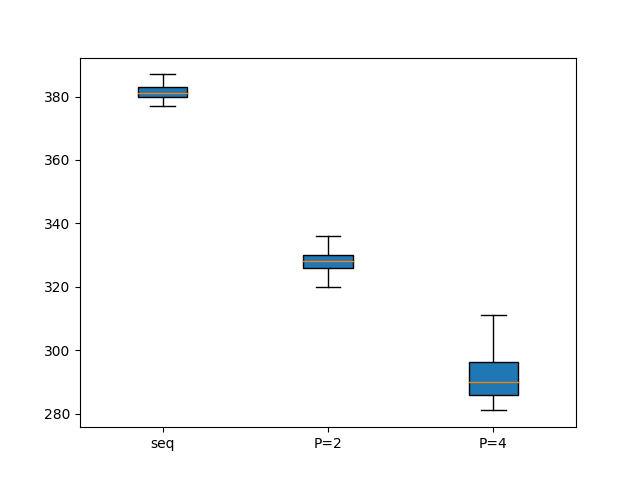
\includegraphics[width=0.7\linewidth]{Preset_2}
	\caption[Preset1]{Preset2}
	\label{fig:preset2}
\end{figure}

\begin{figure}
	\centering
	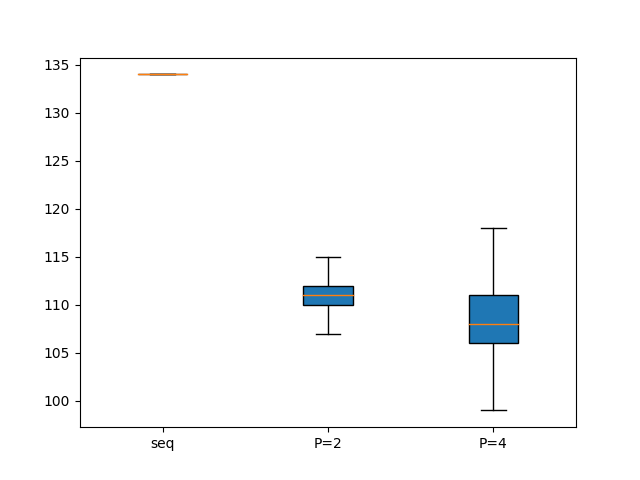
\includegraphics[width=0.7\linewidth]{Preset_3}
	\caption[Preset1]{Preset3}
	\label{fig:preset3}
\end{figure}

\subsubsection{Overhead}Gegeven dat de overhead per preset x is kunnen we de efficientie bepalen van de parallele implementatie.
De overhead van het verdelen in threads in niet aanwezig bij de sequentiele versie omdat de sequentiele versie niet opdeeld in kleine taken.
De overhead zou verminderd kunnen worden door een cutoof te gebruiken.
De overhead is verschillend per preset omdat het opdelen van het werk afhangt van de respectievelijke data.
\subsubsection{Speed-up}
Een perfecte speed-up zou gelijk zijn aan het aantal extra processors, dit is hier niet het geval...
Schaalt de berekening voor meer cores?
\subsection{Fase 2}





\end{document}
